\documentclass[12pt, a4paper]{article}

\usepackage[italian]{babel}
\usepackage{geometry}
\usepackage{amsmath}
\usepackage{amssymb}
\usepackage{graphicx}
\usepackage{ulem}
\geometry{margin=1cm}
\usepackage{listings}
\usepackage{xparse}
\usepackage{expl3}
\usepackage{tikz}
\usetikzlibrary{calc}
\usepackage{xcolor}
\let\olditemize\itemize
\renewcommand\itemize{\olditemize\setlength\itemsep{0em}}

\definecolor{codegreen}{rgb}{0,0.6,0}
\definecolor{codegray}{rgb}{0.5,0.5,0.5}
\definecolor{codepurple}{rgb}{0.58,0,0.82}
\definecolor{backcolour}{rgb}{0.95,0.95,0.92}

\lstdefinestyle{mystyle}{
    backgroundcolor=\color{backcolour},   
    commentstyle=\color{codegreen},
    keywordstyle=\color{magenta},
    numberstyle=\tiny\color{codegray},
    stringstyle=\color{codepurple},
    basicstyle=\ttfamily\footnotesize,
    breakatwhitespace=false,         
    breaklines=true,                 
    captionpos=b,                    
    keepspaces=true,                 
    numbers=left,                    
    numbersep=5pt,                  
    showspaces=false,                
    showstringspaces=false,
    showtabs=false,                  
    tabsize=2
}

\lstset{style=mystyle}

\newcommand{\tikzmark}[1]{\tikz[baseline,remember picture] \coordinate (#1) {};}
\newcommand{\bra}[1]{\langle #1 |}
\newcommand{\ket}[1]{| #1 \rangle}
\newcommand{\customfbox}[1]{
    \begin{center}
        \noindent\fbox{\parbox{\dimexpr\linewidth-2\fboxsep-2\fboxrule\relax}{\centering #1}}
    \end{center}
    }
\ExplSyntaxOn
\NewDocumentCommand{\braket}{m O{} m}{ \langle #1 | \tl_if_blank:nTF {#2} {#3} {#2|#3} \rangle }
\ExplSyntaxOff

\title{Relazione Home Assignment 8}
\author{Daniele Sacco (5616921), Daniele Scaffai (5658260), Lorenzo Vaccarecci (5462843)}
\date{}

\begin{document}
\maketitle
\section*{Obiettivo}
L'obiettivo di questo Home Assignment è l'implementazione del protocollo degli errori di Shor, in particolare gli errori di tipo bit flip, phase flip e small error.
\section*{Bit flip}
\section*{Svolgimento}
Abbiamo riprodotto, usando qiskit, il circuito che è stato fornito dal docente. Tra le due barriere viene applicata la porta di Pauli $X$ per simulare il bit flip.
\begin{lstlisting}[language={Python}]
psi = QuantumRegister(1, 'psi')
ancilla = AncillaRegister(8, 'ancilla')
c_reg = ClassicalRegister(1, 'c_reg')
qc_x_gate = QuantumCircuit(psi, ancilla, c_reg)

qc_x_gate.cx(psi[0],ancilla[2])
qc_x_gate.cx(psi[0],ancilla[5])

qc_x_gate.h(psi[0])
qc_x_gate.h(ancilla[2])
qc_x_gate.h(ancilla[5])

qc_x_gate.cx(psi[0],ancilla[0])
qc_x_gate.cx(ancilla[2],ancilla[3])
qc_x_gate.cx(ancilla[5],ancilla[6])

qc_x_gate.cx(psi[0],ancilla[1])
qc_x_gate.cx(ancilla[2],ancilla[4])
qc_x_gate.cx(ancilla[5],ancilla[7])

qc_x_gate.barrier()
qc_x_gate.x(psi[0])
qc_x_gate.barrier()

qc_x_gate.cx(psi[0],ancilla[0])
qc_x_gate.cx(ancilla[2],ancilla[3])
qc_x_gate.cx(ancilla[5],ancilla[6])

qc_x_gate.cx(psi[0],ancilla[1])
qc_x_gate.cx(ancilla[2],ancilla[4])
qc_x_gate.cx(ancilla[5],ancilla[7])

qc_x_gate.ccx(ancilla[1],ancilla[0],psi[0])
qc_x_gate.ccx(ancilla[4],ancilla[3],ancilla[2])
qc_x_gate.ccx(ancilla[7],ancilla[6],ancilla[5])

qc_x_gate.h(psi[0])
qc_x_gate.h(ancilla[2])
qc_x_gate.h(ancilla[5])

qc_x_gate.cx(psi[0],ancilla[2])
qc_x_gate.cx(psi[0],ancilla[5])
qc_x_gate.ccx(ancilla[5],ancilla[2],psi[0])

qc_x_gate.measure(psi[0], c_reg[0])
qc_x_gate.draw(output='mpl')

simulator = AerSimulator()

job = simulator.run(qc_x_gate, shots=2048)
result = job.result()

counts = result.get_counts(qc_x_gate)
print(counts)

labels = list(counts.keys())
values = list(counts.values())

fig, ax = plt.subplots(figsize=(8, 4))

bars = ax.bar(labels, values, color='#c4a287')

ax.set_ylabel('Conteggi')
ax.set_title('Risultati della simulazione quantistica')
ax.set_ylim(0, max(values) * 1.1)

plt.show()
\end{lstlisting}
\begin{center} 
        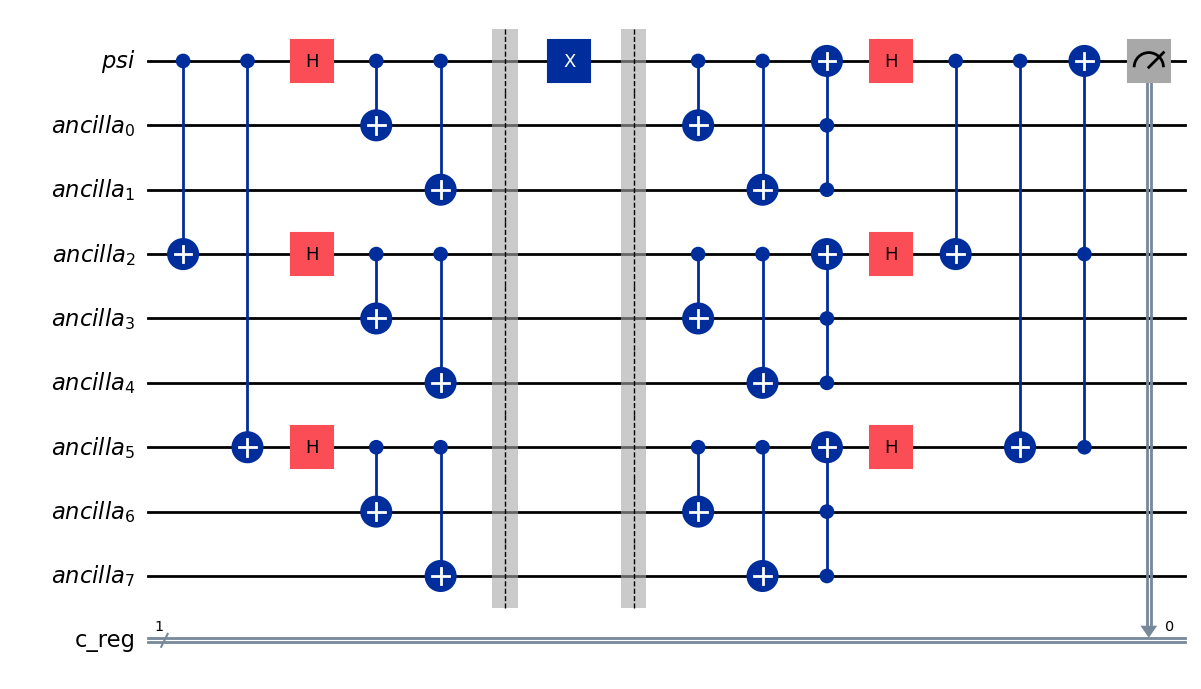
\includegraphics[width=0.6\textwidth]{img/circuit.png} 
        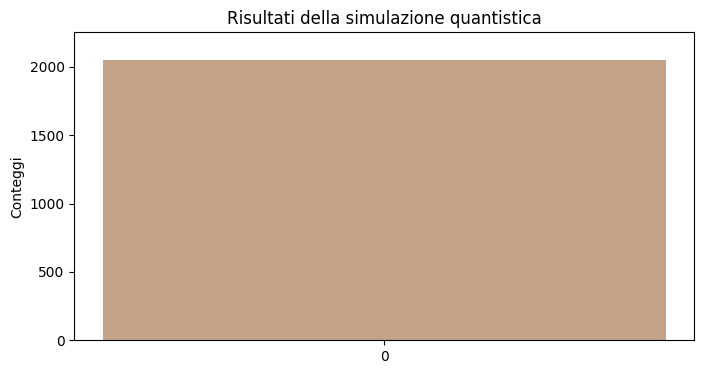
\includegraphics[width=0.4\textwidth]{img/resultsSuccess.png}
\end{center}

\section*{Phase flip}
\section*{Svolgimento}
Abbiamo riprodotto, usando qiskit, il circuito che è stato fornito dal docente. Tra le due barriere viene applicata la porta di Pauli $Z$ per simulare il phase flip.
\begin{lstlisting}[language={Python}]
psi = QuantumRegister(1, 'psi')
ancilla = AncillaRegister(8, 'ancilla')
c_reg = ClassicalRegister(1, 'c_reg')
qc_z_gate = QuantumCircuit(psi, ancilla, c_reg)

qc_z_gate.cx(psi[0],ancilla[2])
qc_z_gate.cx(psi[0],ancilla[5])

qc_z_gate.h(psi[0])
qc_z_gate.h(ancilla[2])
qc_z_gate.h(ancilla[5])

qc_z_gate.cx(psi[0],ancilla[0])
qc_z_gate.cx(ancilla[2],ancilla[3])
qc_z_gate.cx(ancilla[5],ancilla[6])

qc_z_gate.cx(psi[0],ancilla[1])
qc_z_gate.cx(ancilla[2],ancilla[4])
qc_z_gate.cx(ancilla[5],ancilla[7])

qc_z_gate.barrier()
qc_z_gate.z(psi[0])
qc_z_gate.barrier()

qc_z_gate.cx(psi[0],ancilla[0])
qc_z_gate.cx(ancilla[2],ancilla[3])
qc_z_gate.cx(ancilla[5],ancilla[6])

qc_z_gate.cx(psi[0],ancilla[1])
qc_z_gate.cx(ancilla[2],ancilla[4])
qc_z_gate.cx(ancilla[5],ancilla[7])

qc_z_gate.ccx(ancilla[1],ancilla[0],psi[0])
qc_z_gate.ccx(ancilla[4],ancilla[3],ancilla[2])
qc_z_gate.ccx(ancilla[7],ancilla[6],ancilla[5])

qc_z_gate.h(psi[0])
qc_z_gate.h(ancilla[2])
qc_z_gate.h(ancilla[5])

qc_z_gate.cx(psi[0],ancilla[2])
qc_z_gate.cx(psi[0],ancilla[5])
qc_z_gate.ccx(ancilla[5],ancilla[2],psi[0])

qc_z_gate.measure(psi[0], c_reg[0])

qc_z_gate.draw(output='mpl')

simulator = AerSimulator()

job = simulator.run(qc_z_gate, shots=2048)
result = job.result()

counts = result.get_counts(qc_z_gate)
print(counts)

labels = list(counts.keys())
values = list(counts.values())

fig, ax = plt.subplots(figsize=(8, 4))

bars = ax.bar(labels, values, color='#c4a287')

ax.set_ylabel('Conteggi')
ax.set_title('Risultati della simulazione quantistica')
ax.set_ylim(0, max(values) * 1.1)

plt.show()
\end{lstlisting}
\begin{center} 
        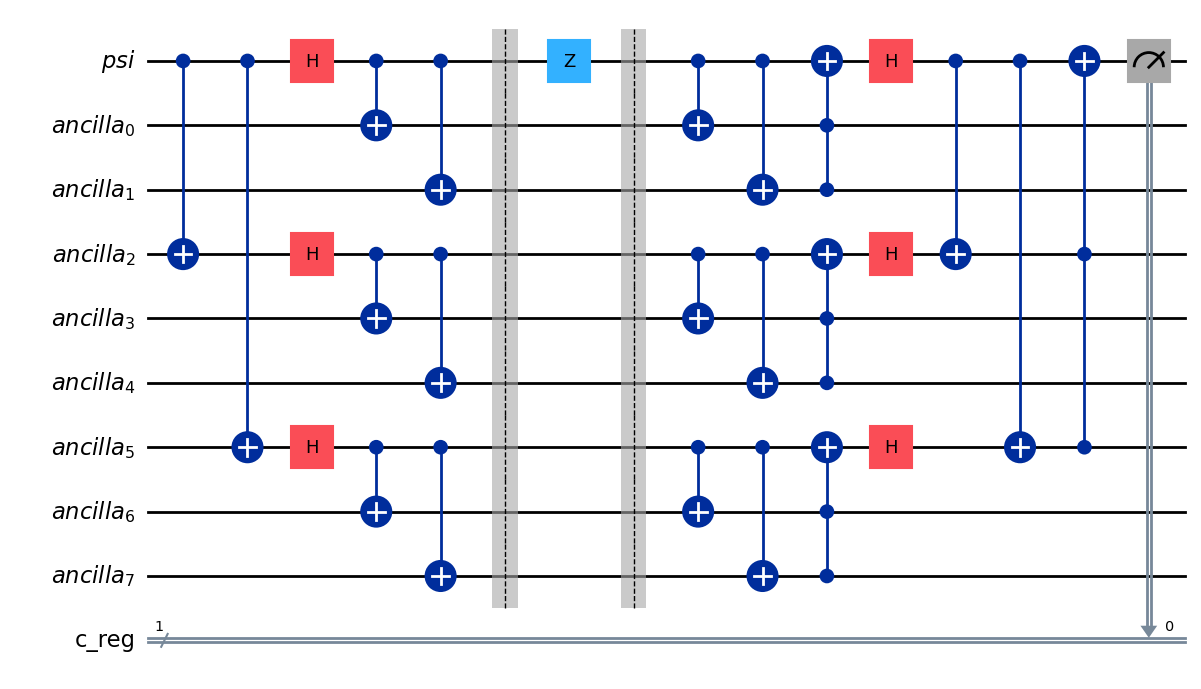
\includegraphics[width=0.6\textwidth]{img/circuitPhaseflip.png} 
        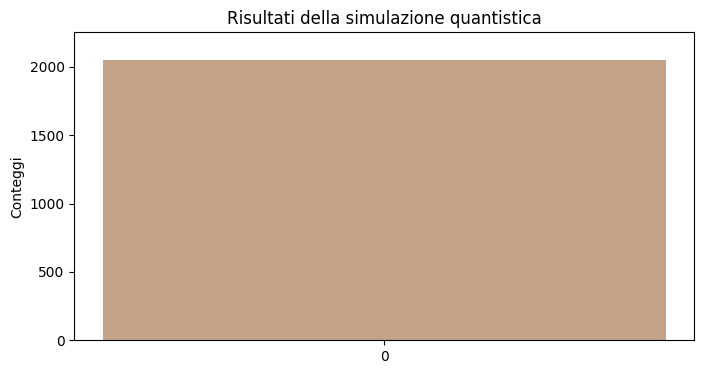
\includegraphics[width=0.4\textwidth]{img/resultsSuccessPhaseflip.png}
\end{center}

\section*{Small error}
\section*{Svolgimento}
Abbiamo riprodotto, usando qiskit, il circuito che è stato fornito dal docente. Tra le due barriere viene applicata una piccola rotazione sull'asse delle $x$ a $\ket{\psi}$ per simulare uno small error.
\begin{lstlisting}[language={Python}]
psi = QuantumRegister(1, 'psi')
ancilla = AncillaRegister(8, 'ancilla')
c_reg = ClassicalRegister(1, 'c_reg')
qc_rx_gate = QuantumCircuit(psi, ancilla, c_reg)

qc_rx_gate.cx(psi[0],ancilla[2])
qc_rx_gate.cx(psi[0],ancilla[5])

qc_rx_gate.h(psi[0])
qc_rx_gate.h(ancilla[2])
qc_rx_gate.h(ancilla[5])

qc_rx_gate.cx(psi[0],ancilla[0])
qc_rx_gate.cx(ancilla[2],ancilla[3])
qc_rx_gate.cx(ancilla[5],ancilla[6])

qc_rx_gate.cx(psi[0],ancilla[1])
qc_rx_gate.cx(ancilla[2],ancilla[4])
qc_rx_gate.cx(ancilla[5],ancilla[7])

qc_rx_gate.barrier()
qc_rx_gate.rx(np.pi/8, psi[0])
qc_rx_gate.barrier()

qc_rx_gate.cx(psi[0],ancilla[0])
qc_rx_gate.cx(ancilla[2],ancilla[3])
qc_rx_gate.cx(ancilla[5],ancilla[6])

qc_rx_gate.cx(psi[0],ancilla[1])
qc_rx_gate.cx(ancilla[2],ancilla[4])
qc_rx_gate.cx(ancilla[5],ancilla[7])

qc_rx_gate.ccx(ancilla[1],ancilla[0],psi[0])
qc_rx_gate.ccx(ancilla[4],ancilla[3],ancilla[2])
qc_rx_gate.ccx(ancilla[7],ancilla[6],ancilla[5])

qc_rx_gate.h(psi[0])
qc_rx_gate.h(ancilla[2])
qc_rx_gate.h(ancilla[5])

qc_rx_gate.cx(psi[0],ancilla[2])
qc_rx_gate.cx(psi[0],ancilla[5])
qc_rx_gate.ccx(ancilla[5],ancilla[2],psi[0])

qc_rx_gate.measure(psi[0], c_reg[0])

qc_rx_gate.draw(output='mpl')

simulator = AerSimulator()

job = simulator.run(qc_rx_gate, shots=2048)
result = job.result()

counts = result.get_counts(qc_rx_gate)
print(counts)

labels = list(counts.keys())
values = list(counts.values())

fig, ax = plt.subplots(figsize=(8, 4))

bars = ax.bar(labels, values, color='#c4a287')

ax.set_ylabel('Conteggi')
ax.set_title('Risultati della simulazione quantistica')
ax.set_ylim(0, max(values) * 1.1)

plt.show()
\end{lstlisting}
\begin{center} 
        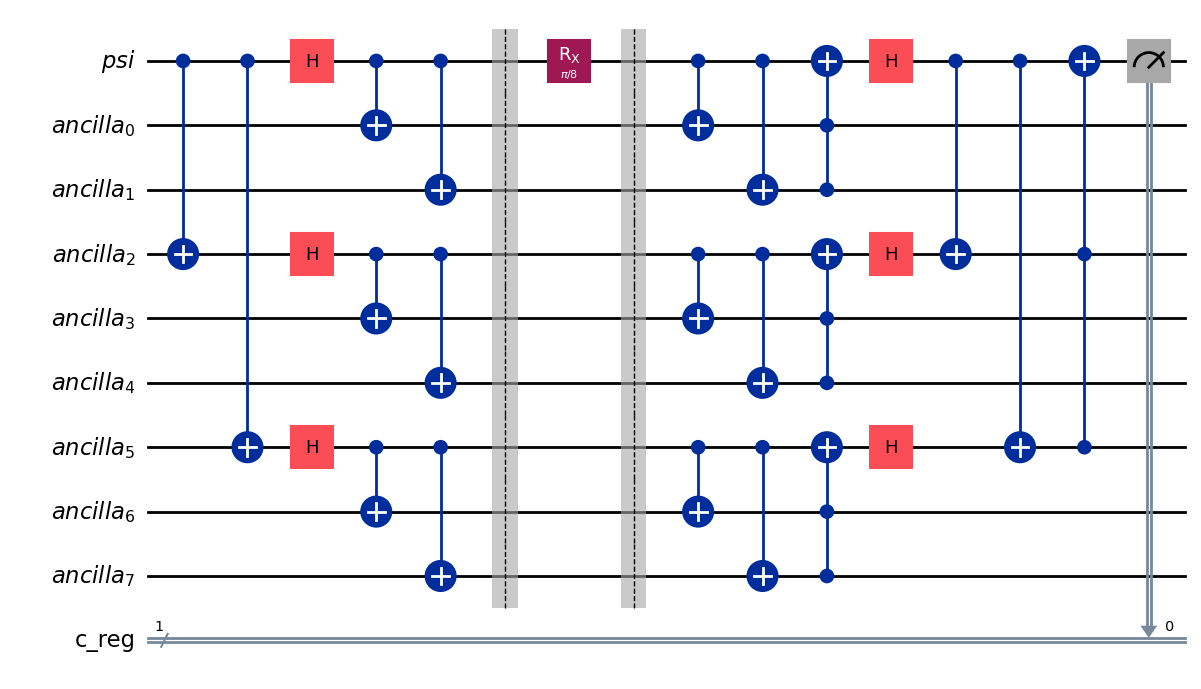
\includegraphics[width=0.6\textwidth]{img/circuitSmallError.png} 
        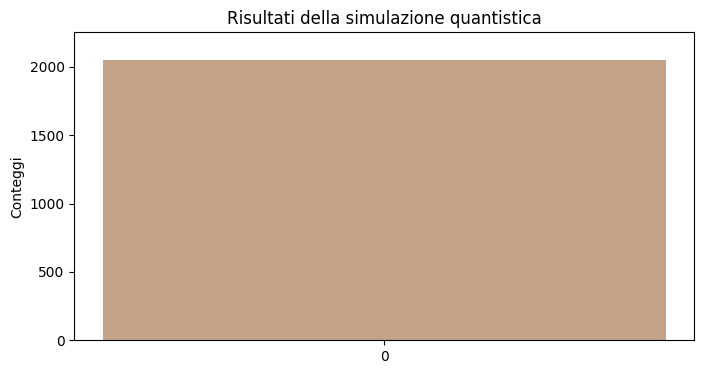
\includegraphics[width=0.4\textwidth]{img/resultsSuccessSmallError.png}
\end{center}

\section*{Risultati}
E' stato aggiunto un misuratore alla fine di ogni circuito e sono state eseguite 2048 simulazioni per ciascuno. La misura attesa per ogni tipo di errore è 0, perchè è lo stato iniziale di $\ket{\psi}$.

\section*{Conclusioni}
I risultati ottenuti corrispondono a quelli attesi, quindi possiamo concludere che l'implementazione del protocollo di correzione degli errori di Shor è corretta.

\end{document}